\documentclass[aspectratio=169]{beamer}

\usetheme{Madrid}
\usecolortheme{whale}

% Remove navigation symbols to make it look clean like the friend's
\setbeamertemplate{navigation symbols}{}

\usepackage{graphicx}
\usepackage{booktabs}
\usepackage{tikz}

\title{3D Symbolic Region Puzzle}
\subtitle{A Non-Planar Symbolic Polycube Challenge}
\author{Odan Lafrance \and Abdelouahad Alla}
\institute{University of Mons --- KRR 2026}
\date{May 2026}

\begin{document}

\begin{frame}
    \titlepage
\end{frame}

\begin{frame}{A 3D Instance}
    \begin{columns}
        \column{0.45\textwidth}
        \centering
        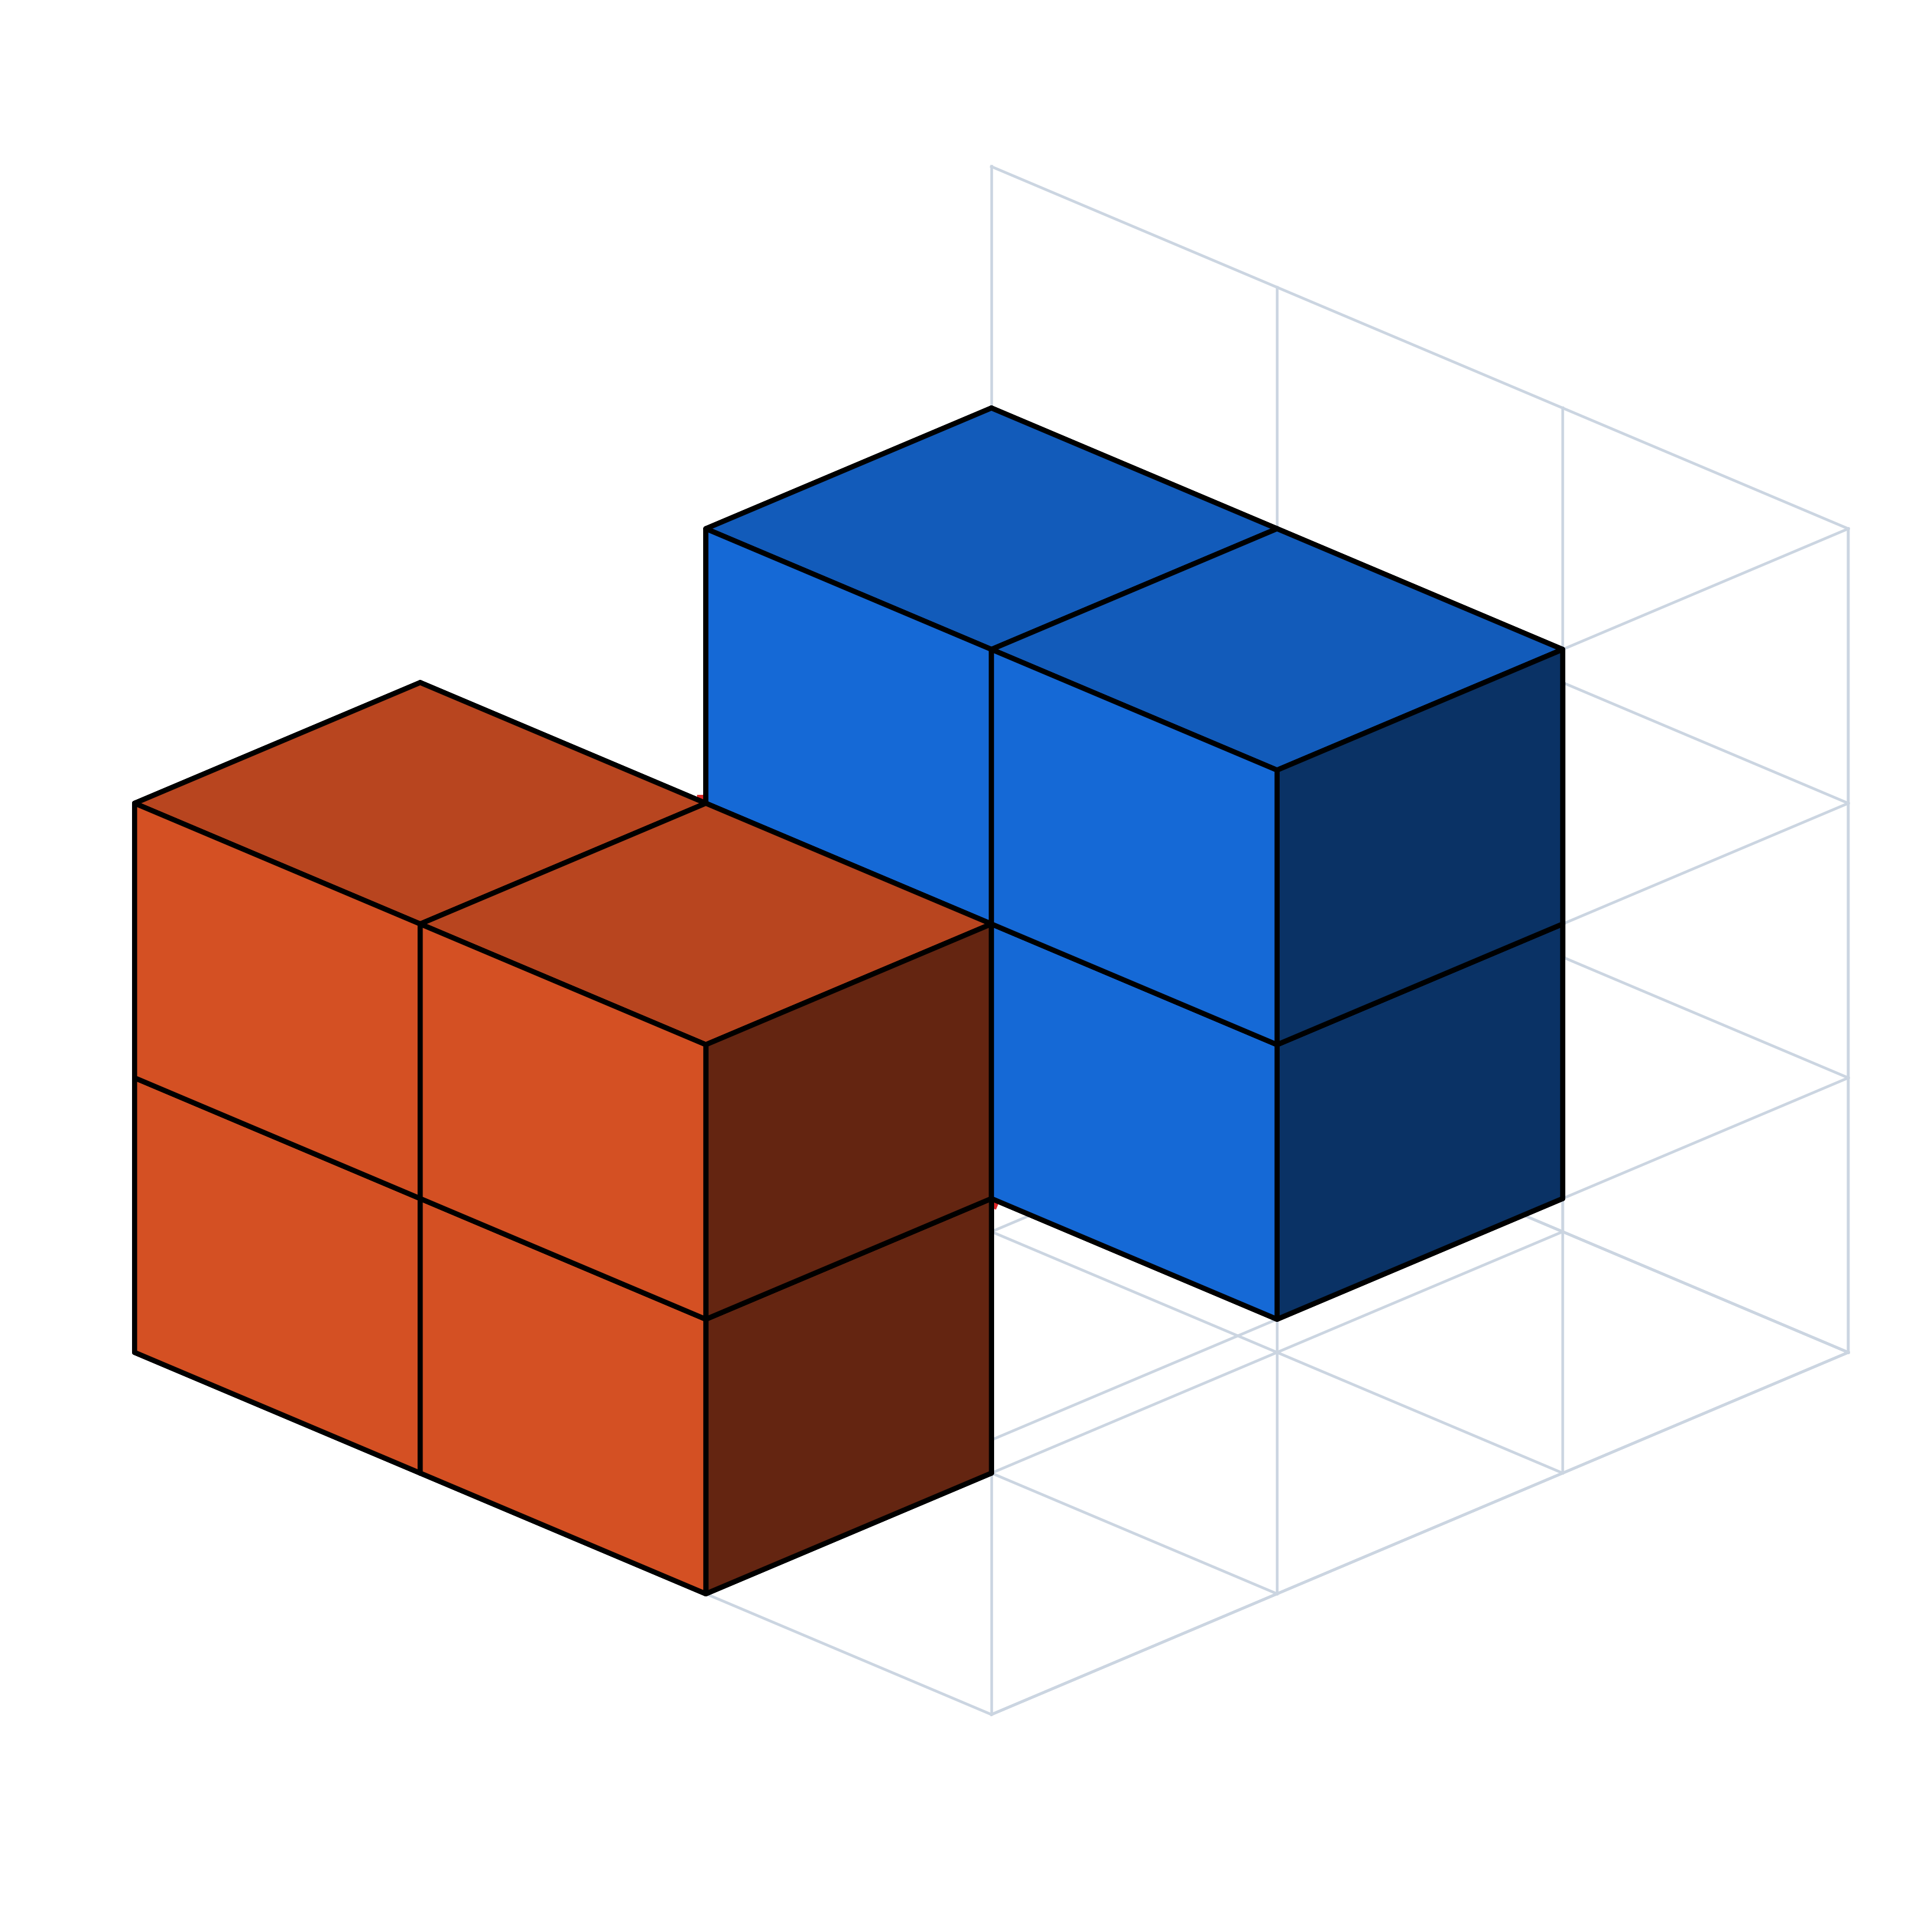
\includegraphics[width=\textwidth]{result_pro.png}\\
        \vspace{0.2cm}
        \textit{View A: Non-Planar Instance}
        
        \column{0.55\textwidth}
        \textbf{Puzzle characteristics:}
        \begin{itemize}
            \item \textbf{Goal:} Partition a polycube of $c$ unit cubes into exactly $m$ non-planar regions without boundary violation.
            \item \textbf{Given:} 
            \begin{itemize}
                \item A 3D board shape
                \item A finite set of drawn symbols $\Sigma$
                \item Physical walls $W$
            \end{itemize}
            \item \textbf{Method: Answer-set programming} (Clingo): Guess partition regions, compute spatial bounds, check constraints iteratively.
        \end{itemize}
    \end{columns}
\end{frame}

\begin{frame}{Puzzle Overview --- Motivation}
    \textbf{Why ASP?}
    \begin{itemize}
        \item Checking a candidate topological placement is fast.
        \item Finding a correct structural placement is hard (combinations blow up).
        \item[$\Rightarrow$] ASP is a natural fit.
    \end{itemize}
    \vspace{0.5cm}
    \textbf{Puzzle input}
    \begin{itemize}
        \item Board geometry: Total cells $c=12$, Boundaries $N=4$.
        \item Sub-constraints: Number of regions $m$, classes of symbols $k$, walls $|W|$.
    \end{itemize}
    \vspace{0.5cm}
    \textbf{Goal}
    \begin{itemize}
        \item Place non-planar partitions in the $c$-cube grid without geometric mismatch.
        \item Make the partitions strictly contain exactly one of each symbol $\Sigma$.
    \end{itemize}
    \vspace{0.5cm}
    \tiny{\textcolor{gray}{Context: Inspired by 3D polycube constraints and Golomb's original logic designs (1994).}}
\end{frame}

\begin{frame}{Puzzle Overview --- The Constraints}
    \begin{columns}
        \column{0.5\textwidth}
        \textbf{Rules properties:}
        \begin{itemize}
            \item \textbf{Non-planar} --- Not a flat ``plate'' of cubes, must expand across x, y, z individually per region!
            \item \textbf{Connectivity} --- Pure spatial graph adjacency required.
            \item \textbf{Symbol Completeness} --- A region acts as a strict container.
            \item \textbf{Wall Separation} --- If a wall falls between two blocks, they belong to disjoint regions.
        \end{itemize}
        
        \column{0.5\textwidth}
        \centering
        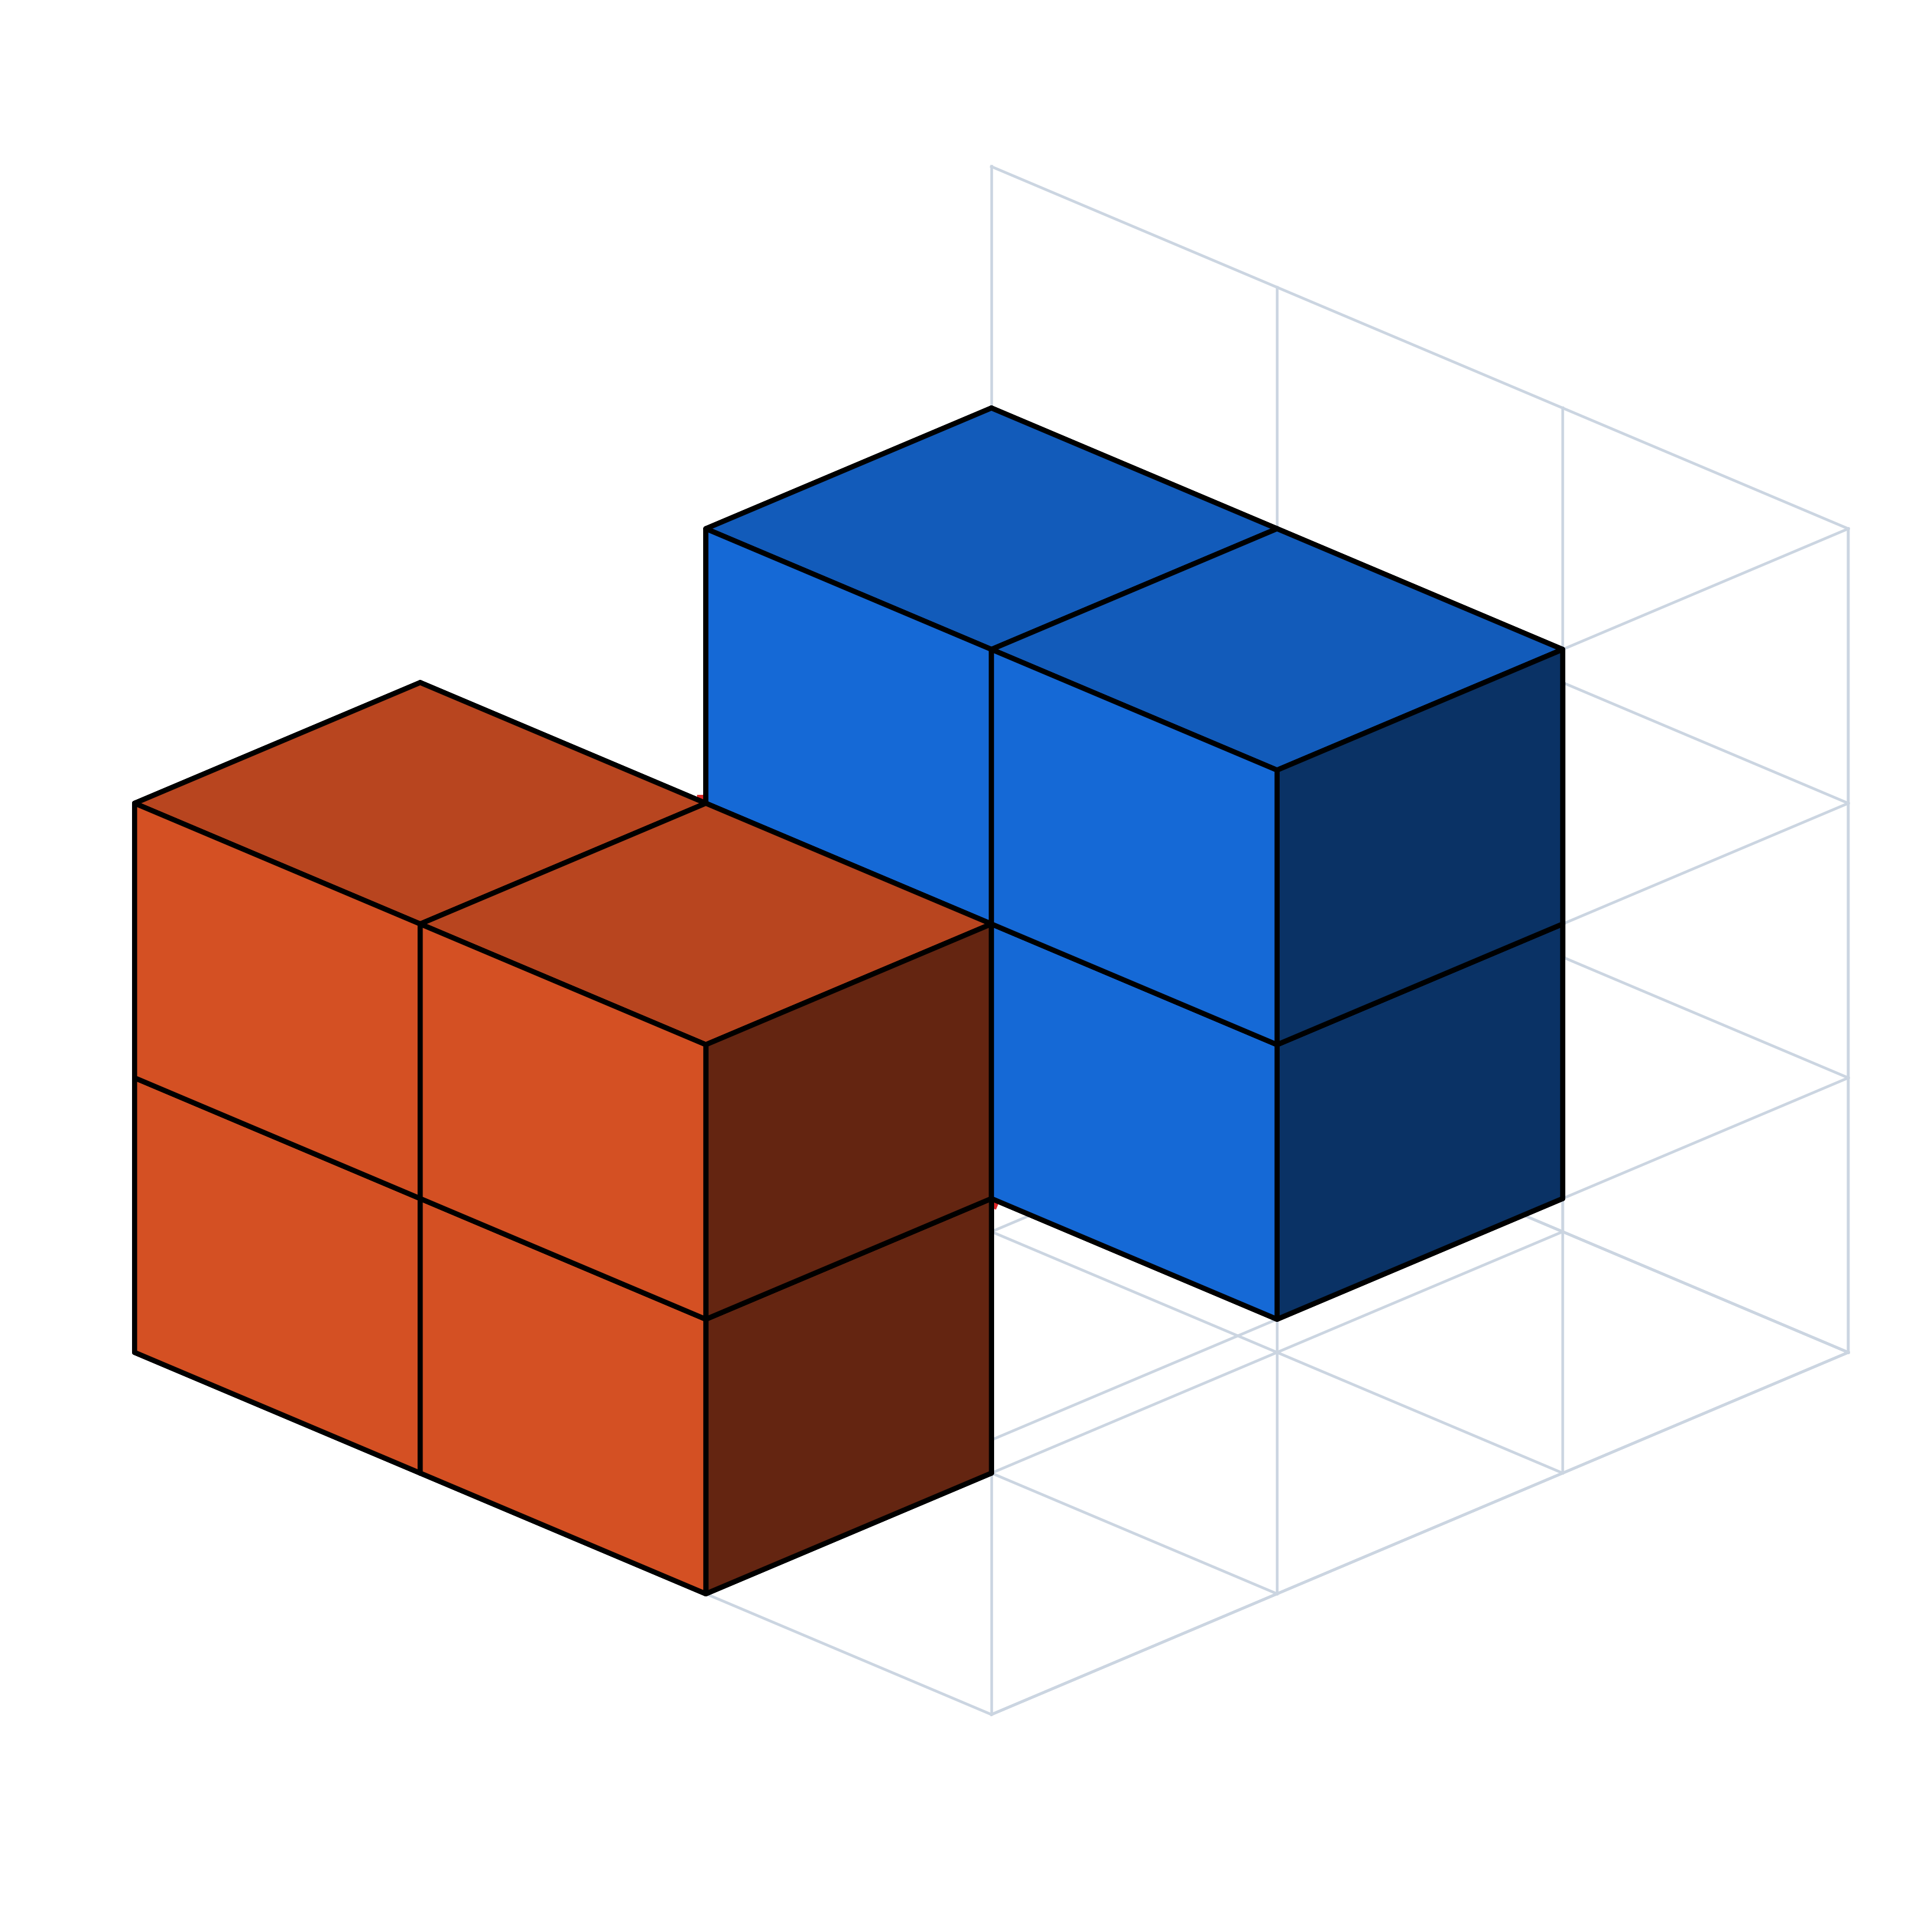
\includegraphics[width=0.8\textwidth]{result_pro.png}\\
        \vspace{0.2cm}
        \footnotesize{\textbf{Chirality / Volume matters here:}\\ This instance needs specific topological growth to avoid trapping uncolored cells.}
    \end{columns}
\end{frame}

\begin{frame}{Puzzle Overview --- Game Rules \& Experience}
    \textbf{Input:}
    \begin{itemize}
        \item Grid limits $N$, target size $c$.
        \item Visual markers (e.g., $\bigstar, \bullet$) attached to unit shapes.
    \end{itemize}
    \vspace{0.3cm}
    \textbf{Objective:}
    Place boundaries defining exactly $m$ non-planar polycubes encapsulating everything.
    \vspace{0.3cm}
    \textbf{Physical verification:}
    \begin{itemize}
        \item \textbf{Transparent/Painted Blocks} on tables.
        \item Check visually from outside (symbols always outward-facing).
        \item No tools, no breaking pieces. Done in seconds.
    \end{itemize}
    \vspace{0.3cm}
    \textbf{Why difficult:} One single bad region placement starves surrounding adjacent cells of space, collapsing the entire grid recursively.
\end{frame}

\begin{frame}{ASP Model}
    \textbf{Program split:}
    \begin{itemize}
        \item \textbf{Map Generator}: Carves valid boards, places $c$ cubes iteratively ensuring initial topological soundness and global bounding dimensions $N$.
        \item \textbf{Core solver} (guess / connect / prune).
    \end{itemize}
    \vspace{0.3cm}
    \textbf{ASP Logical Pipeline:}
    \begin{enumerate}
        \item \textbf{Guess:} One region ID per independent cube coordinate.
        \item \textbf{Compute:} Breadth-first graph expansion checking adjacent ID similarities.
        \item \textbf{Check:} Count spatial bounding box limits \textit{per} aggregate ID (if $\Delta z=0$, then prune). Verify exactly $1$ symbol class $k$ exists inside the aggregate ID. Identify overlapping walls.
    \end{enumerate}
\end{frame}

\begin{frame}{Experiments \& Complexity Checks}
    \begin{columns}
        \column{0.45\textwidth}
        \textbf{Setup:} clingo 5.4+ $\cdot$ Apple Silicon
        \vspace{0.2cm}\\
        \begin{tabular}{lccc}
            \toprule
            $c$ & $m\times k$ & Walls & Mean \\
            \midrule
            8 & 4 & 2 & 0.0007 s \\
            10 & 4 & 2 & 0.0010 s \\
            12 & 6 & 3 & 0.0016 s \\
            14 & 6 & 3 & 0.0015 s \\
            16 & 8 & 4 & 0.0012 s \\
            \bottomrule
        \end{tabular}
        \vspace{0.3cm}
        
        \textbf{Key points:}
        \begin{itemize}
            \item Heavily constrained rules lead to massive pruning.
            \item SAT extremely fast (fraction of ms) because the search tree is tight.
        \end{itemize}
        
        \column{0.55\textwidth}
        \centering
        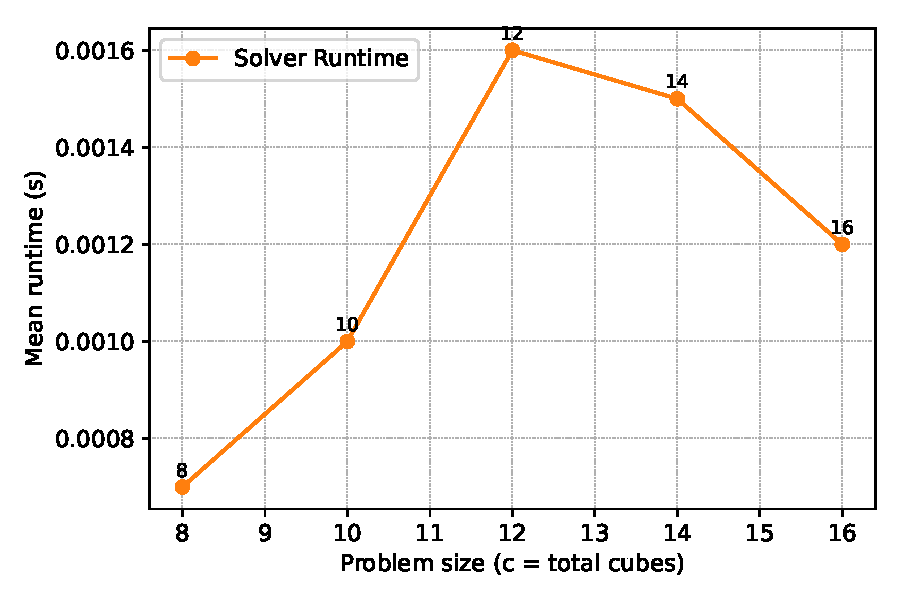
\includegraphics[width=0.9\textwidth]{solver_linear.pdf}\\
        \vspace{0.2cm}
        \textit{Scaling of Core Solver Search Time}
    \end{columns}
\end{frame}

\begin{frame}{Results and Conclusion}
    \begin{columns}
        \column{0.5\textwidth}
        \textbf{Complexity Analysis}
        \begin{itemize}
            \item $\in$ NP (polynomial visual check)
            \begin{itemize}
                \item Connectivity check is $O(c)$.
                \item Non-planarity aggregates in $O(c)$.
                \item Wall bounding is $O(|W|)$.
            \end{itemize}
            \item Scales exponentially for random generation (generator constraints are incredibly sparse).
        \end{itemize}
        \vspace{0.3cm}
        \textbf{Variants}
        \begin{itemize}
            \item \textbf{Size hints:} Adding Fillomino-like region size parameters.
        \end{itemize}
        
        \column{0.5\textwidth}
        \textbf{Take-away}
        \begin{enumerate}
            \item \textbf{Physical}: 3D printable, visually appealing.
            \item \textbf{Verify}: Readily visible logic faces.
            \item \textbf{Clingo}: Outstanding at recursively mapping non-trivial geometry intersections immediately.
        \end{enumerate}
        \vspace{0.5cm}
        \textbf{Next}
        \begin{itemize}
            \item Extend map scale $>32$ cubes.
            \item Test optimization functions for solver symmetry breaking.
        \end{itemize}
    \end{columns}
\end{frame}

\end{document}
